\section{Introduction}
%\KZ{What's the definition of term? What is term similarity? Explain briefly the diff between
%similarity and relatedness. Why is term similarity important?}
%\KZ{One problem is that we don't handle verbs or adjectives. We
%need to point this out either in the title or somewhere here.}

Measuring semantic similarity between terms is a fundamental problem
in lexical semantics \cite{Budanitsky:2006} and it finds many
applications in web and document search \cite{WangLWZ12:Concept}, question and answer systems,
and other text analytics and text understanding scenarios.  By {\em
  terms}, we mean either single words or multi-word expressions
(MWEs).
%{\color{red}in this paper, we refer terms as the collective
%concepts and entities}.
We say two terms are semantically similar, if their
meanings are close, or the concept or object that they represent share many common attributes.  For example, ``emerging markets'' and
``developing countries'' are similar because their semantic contents (the subset of countries) are very similar. Another example, ``Google'' and
``Microsoft'' are similar because they are both software companies. %  and
% as a software company, they share a number of commonalities.
However, ``car'' and ``journey'' are not semantically similar but {\it related} because ``car'' is a transport means for
  the activity ``journey''. Specifically, semantic
similarity is defined by some measure of {\em distance} between two terms on an isA taxonomy.
%which organizes terms by {\em synonymy} and {\em hypernumy} relations.
% Such distance can be either a naive metric of number of distinct edges
% (hops) between two nodes on the taxonomy graph, or more sophisticated
% statistical measures.
It is clear that ``car'' and ``journey'' are quite far away from each other in an isA taxonomy from WordNet as shown in Figure~\ref{fig:tree}.
Semantic similarity is a more specific relationship and is much harder to model than {\em relatedness} (which can be modeled by term
co-occurrence).
% In this paper, we are concerned
% with the efficient computation of semantic similarity between two
% terms.
\begin{figure}[th]
 \centerline{
 \includegraphics[width=0.5\textwidth]{car-journey.eps}}
\caption{A fragment from WordNet showing semantic distance between ``car'' and ``journey''}
\label{fig:tree}
\end{figure}
%\KZ{Include a graph cut from wordNet that shows the distance between
%car and journey.}

%Semantic similarity is different from semantic relatedness.
% Contrary to the semantic relatedness relying on the more general relationships (e.g., part-of and the co-occurrence), semantic similarity relies on the degree of taxonomic
%likeness between concepts considering relationships such as hyponymy and hyperonymy, but most of the semantic similarity measurement methods can be adapted and generalized to deal with semantic relatedness.
%We can adapt and generalize the semantic similarity measurement methods to deal with semantic relatedness, but we cannot adapt the semantic relatedness measurement methods to deal with semantic similarity. For example, \emph{journey} and \emph{car} has a high semantic relatedness score due to the higher co-occurrences in the corpus, while its semantic similarity should be lower because they belong to the different concepts.


%\KZ{Briefly state the existing approaches. Classify them into two categories. State why they don't work for some
%examples. Use concrete examples (challenge 1-3) from the slides to
%illustrate the challenges.}
% Computing the semantic similarity between two terms is tantamount to
% computing the similarity between their {\em contexts}.
Recent work on term similarity can be roughly classified into two main categories: {\em knowledge based} and {\em corpus based}. Knowledge based
approaches rely on handcrafted resources such as thesauri, taxonomies or encyclopedias, as the context of comparison.  Most work in this space
\cite{Rada:1989, Resnik:1995, Agirre:2010} depends on the semantic isA relations in WordNet \cite{Miller1995} which is a manually curated
lexicon and taxonomy. Corpus based approaches work by extracting the contexts of the terms from large corpora and then inducing the
distributional properties of {\em words} or {\em
  n-grams}.
%{\color{red}(It also include the term co-occurrence based method)}.
Corpus can be anything from web pages, web
search snippets to other text repositories.
%For example, Google distance \cite{Cilibrasi:Google} is
%derived from the number of hits returned by the Google search engine.
%Other corpus-based measures rely on the
%content of search results or search snippets.

One significant challenge faced by the knowledge-based methods is the
limited coverage of taxonomies such as WordNet (with 155,287 words
at last count).
%Through two decades of development, the most recent release
%of WordNet (version 3.0) contains
%155,287 words organized in 117,659 synsets and 206,941 word-sense pairs.
It does not cover many proper nouns (e.g., ``Microsoft''
or ``Google''), or very popular senses (e.g., Apple the company or
Jaguar the car make). Another major restriction of WordNet is that it
primarily covers single words with only a handful of phrases or
multi-word expressions.  For example, it does not know ``General
Electric'' or ``emerging markets''.
%Thus, it is impossible for these
%WordNet-based methods to correctly compute the semantic similarity
%which involves these unknown terms or terms with unknown senses.
Consequently, the similarity between ``General Electric'' and ``GE''
is completely ignored.
%they are exactly the same thing.
%With today's fast changing world, it is just not possible for manually
%curated lexical databases like WordNet to keep up with the pace of the
%creation of new words and phrases in human languages.
%
%Meanwhile, new words are constantly being
%created on the Web as well as new senses are assigned to existing words,
%it is also costly for manually maintaining existing thesauri like
%WordNet to capture these new words and senses if not impossible.

Corpus-based approaches also face several serious limitations.
First, such measures are biased because of the indexing and 
ranking mechanisms used in search engines. 
% Unfortunately, these mechanisms are often ``commercial
% secrets'' and are opaque to outsiders.
For example when querying the term ``date''
%\footnote{sense 1: day of the month; ...; sense 8: sweet edible fruit of the
%date palm with a single long woody seed.}
or ``range''
%\footnote{sense 1: scope; ...; sense 9: stove, kitchen stove. Senses of
%``date'' and ``range'' mentioned above are annotated in WordNet.}
on Google, none of the first 100 results has anything to do with
fruits (a sense for date) or cooking stoves (a sense for range),
because these are rare senses of the two terms.
%and are considered not ``relevant'' by Google.
With such search results, it is not surprising that a corpus-based
method would think ``asian pear'' and ``date'' share very little commonality.
%and ``food processor'' and ``range'' are very different, too.
Second, some search-result oriented similarity methods require
interaction with the search engine which has high communication overhead
and high index costs, and are not suitable for online applications.
%Hence they are not suitable for online applications which require fast
%response time.
%For the second distributional context based approach, in order to
%extend the data coverage, it adopts the search snippets or web documents
%as the corpus. This indicates this approach heavily depends on the
%search engine's ranking algorithm.
Third, statistical distribution based on words or n-grams in the
context ignores the fact that i) the semantic units can be MWEs and not
words, let alone n-grams; and ii) many words or phrases are ambiguous
in meaning. %e.g., ``apple'' can be both a fruit and a company.
%Consequently, distribution thus computed may not truly represent the
%semantic landscape of the contexts. To fix this problem, some methods
%in this category resorted to manual labeling of senses in a machine
%learning approach \cite{Bollegala:2007, Bollegala:Supervised} which is
%tedious and time-consuming.
Finally, corpus-based methods focus on
surrounding context of a term or the co-occurrence of two terms within
a neighborhood, both of which are more suitable to the calculation of
semantic relatedness rather than similarity.  Under this approach,
``car'' and ``journey'' would have high semantic relatedness because
they co-occur very frequently on web texts.
%when in fact they are {\em  not} similar because
%$Apple$ is a company and $iPad$ is a product by the company.

% \begin{figure}[t]
% %\makeatletter\def\@captype{figure}\makeatother
%  \centerline{
%  \includegraphics[width=0.5\textwidth]{Correlation-on-MC-r.eps}}
% \caption{Pearson correlation coefficient in different approaches} \label{fig:Correlation-on-MC}
% \end{figure}
%
% \begin{table}[!h]
% \centering
% \caption{Concept lists of a pairwise term Microsoft and Apple}% (extracted using Hearst patterns)}
% \label{tab:microsoft-apple}
% \begin{tabular}{|l|c|l|c|}\hline
% concepts of Microsoft & weight & concepts of Apple & weight\\\hline
% company   &0.4239 &fruit  &0.2952\\
% u.s. company  &0.0349 &company    &0.1362\\
% large company &0.0321 &seasonal fruit &0.0826\\
% client    &0.0256 &food   &0.0612\\
% organization  &0.0217 &fresh fruit    &0.0389\\
% software giant    &0.0217 &fruit tree &0.0223\\
% international company &0.0207 &brand  &0.0216\\
% provider  &0.0184 &crop   &0.0147\\
% industry leader   &0.0184 &flavor &0.0121\\
% technology company    &0.0145 &manufacturer   &0.0100\\
% software company  &0.0141 &tree   &0.0083\\
% big company   &0.0125 &competitor &0.0077\\
% giant &0.0123 &product    &0.0067\\
% player    &0.0112 &juice  &0.0067\\
% software vendor   &0.0095 &fruit juice    &0.0065\\
% competitor    &0.0086 &snack  &0.0054\\
% partner   &0.0082 &healthy snack  &0.0052\\
% manufacturer  &0.0071 &dried fruit    &0.0051\\
% industry giant    &0.0068 &large company  &0.0048\\
% big player    &0.0063 &tree fruit &0.0048\\
% \hline
% \end{tabular}
% \end{table}
%
% \begin{table}[!h]
% \centering
% \caption{Concept clusters of a pairwise term Microsoft and Apple}% (extracted using Hearst patterns)}
% \label{tab:microsoft-apple-clusters}
% \begin{tabular}{|p{2pt}|l|c|p{2pt}|l|c|}\hline
%  & concepts &  &  & concepts & \\
% id & of Microsoft & weight & id & of Apple & weight\\\hline
% 1 &company    &0.3738 &1  &fruit  &0.2952\\
% 1 &u.s. company   &0.0349 &1  &seasonal fruit &0.0826\\
% 1 &client &0.0256 &1  &tree fruit &0.0048\\
% 1 &large company  &0.0227 &1  &fresh fruit    &0.0389\\
% 1 &software giant &0.0217 &1  &juice  &0.0067\\
%   &international-&    &   &   &\\
% 1 &company    &0.0207 &1  &fruit juice    &0.0065\\
%   &technology-    &   &   &   &\\
% 1 &company    &0.0145 &1  &dried fruit    &0.0051\\
% 1 &software company   &0.0141 &2  &company    &0.1239\\
% 1 &big company    &0.0125 &2  &manufacturer   &0.0100\\
% 1 &giant  &0.0123 &2  &competitor &0.0077\\
% 1 &player &0.0112 &2  &large company  &0.0048\\
% 1 &software vendor    &0.0095 &3  &food   &0.0612\\
% 1 &competitor &0.0086 &3  &snack  &0.0054\\
% 1 &partner    &0.0082 &3  &healthy snack  &0.0052\\
% 1 &manufacturer   &0.0071 &4  &fruit tree &0.0223\\
% 1 &industry giant &0.0068 &4  &tree   &0.0083\\
% 1 &big player &0.0063 &5  &brand  &0.0216\\
% 2 &organization   &0.0217 &6  &crop   &0.0147\\
% 3 &provider   &0.0184 &7  &flavor &0.0121\\
% 4 &industry leader    &0.0184 &8  &product    &0.0067\\
% \hline
% \end{tabular}
% \end{table}

%\KZ{Briefly give the problem statement. Don't talk about the specific challenges below which are details of
%the approach. But briefly mention what is our approach: 1) judge the types of the terms; 2) collect the context
%of the terms by clustering the their sense; 3) compute the similarity.
%Stress that our key difference is 1) the use of a large semantic network extracted from
%very big data which shows  the power of universal knowledge from the web; 2) our approach is very fast
%compared to previous approach because... You can show the similarity result from our system on the few
%difficult examples in the previous paragraph. No need to show detailed tables or figures. Just let the reader
%get an idea of what you can achieve and how accurate your approach is!}

In this paper, we propose a light-weight but effective framework for
computing semantic similarity %(a number between 0 and 1)
between a pair of terms using a large scale, general purpose isA
network obtained from a web corpus. It belongs to the knowledge-based method.
% The framework computes similarity in three simple steps:
% \begin{enumerate}
% \item typecheck the input terms into either an {\em entity} or a {\em concept};
% \item represent the semantic contexts of each term according to its type and its
% position in the isA semantic network and disambiguate the senses of the input
% terms by clustering the super-concepts or the subsumed entities within the
% network;
% \item computing similarity between the probability distribution of the two contexts
% using a max-max similarity function.
% \end{enumerate}
% With this novel approach, we are able to efficiently compute the semantic
% similarity between almost any MWEs. We focus on noun-based terms in this paper
% though the framework can be easily extended to verbs and adjectives as well.
Below is a small sample of results:

\begin{itemize}
\item High similarity (synonyms): \pair{general~ electric}{ge}
%  Synonyms that refer to the same entity should have the highest
%  similarity score.
\item High similarity (ambiguous terms): \pair{microsoft}{apple},
  \pair{orange}{red}
%  \sim{asian pear}{date}  =  0.7111 \\
%  Words such as ``apple'' and ``orange'' have multiple
%  senses. However, when people compare ``apple'' with ``microsoft'',
%  they consider ``apple'' in the sense of a company rather than a
%  fruit, and when they compare ``orange'' and ``red'', they consider
%  ``orange'' as a color rather than a fruit. Thus, disambiguation
%  needs to be performed by default in similarity comparison.

\item Low similarity (though share same hypernyms in WordNet):
\pair{music}{lunch}, \pair{banana}{beef}
%  These pairs of terms are not similar. However, in an isA network,
%  ``music'' and ``lunch'' may both belong to concepts such as
%  ``activity'', and ``banana'' and ``beef'' may both belong to concepts
%  such as ``food''. We may use their distances in a handcrafted
%  taxonomy to measure similarity, but handcrafted taxonomies have low
%  coverage, while distances in large scale, data driven semantic
%  networks are not easy to measure.

\item Low similarity (related but not similar): \pair{apple}{ipad}, \pair{car}{journey}
%  We need to differentiate similarity from relatedness. Here,
%  ``apple'' and ``ipad'', ``car'' and ``journey'' are related, but
%  they are not similar. {\color{red} This is because ``ipad'' is an electronic product of the company ``apple'' while ``car'' is a traffic tool for
%  the activity ``journey'', however, they belong to the different concepts or far away on an isA taxonomy.}
%
\end{itemize}

% \begin{eqnarray*}
% %\sim{General Electric}{GE} &=& 0.9875 \\
% \sim{General Electric}{GE} &=& 1.0\\
% \sim{Microsoft}{Apple} &=& 0.994 \\
% \sim{food processor}{range} & = & 0.6894 \\
% \sim{asian pear}{date} & = & 0.7111 \\
% \sim{apple}{ipad} &=& 0.0167 \\
% \sim{car}{journey} &=& 0.0001
% \end{eqnarray*}

%\begin{itemize}
%\item Large coverage;
%\item More meaningful similarity (e.g., apple and Microsoft);
%\item Lightweight
%\end{itemize}


%We introduce a scalable and effective approach for measuring
%the semantic similarity between terms in this paper.
The main contributions of this paper are:
\begin{itemize}
\item {\em Our approach has better coverage.}
The semantic network behind this approach is one order of magnitude larger
than WordNet in terms of the number of hypern-ym-hyponym relations.
%Unlike existing methods based on WordNet which only measure the similarity between limited number of words,
Our approach computes similarity between almost any two
known noun-based MWEs.
%This is because the knowledge source behind this approach
%is harnessed from billions of web documents.
%millions of terms, and then we compare the
%similarity between their contexts. It could be used to calculate
%semantic similarity between named entities, etc, which are not listed
%in WordNet or other manually compiled thesauri.

\item {\em Our approach produces more meaningful similarity.}
Unlike corpus-based methods which can confuse similarity with relatedness,
this approach calculates similarity by relations induced from an isA semantic
network. It also seeks to disambiguate terms
% with multiple meanings before calculating similarity
and thus excludes noises from irrelevant senses from
the probability distributions.
%As a result, the similarity results are more relevant and reliable.
%We introduce the concept clustering approach on the collected contexts
%given the term to identify its potential senses automatically,
%and then we utilize the term's sense based similarity evaluation
%method to improve the semantic similarity between terms especially
%for ambiguous terms with skewed data distributions of contexts.
%Thus, we can get more meaningful similarity between terms compared
%to the existing methods for semantic similarity.

\item {\em Our approach is lightweight.}  The most expensive
  clustering algorithm is performed offline.
  The remaining similarity function can be efficiently
  computed online. On average, it takes merely 65 milliseconds to
  compute the similarity for a pair of terms.
\end{itemize}

%\subsection{Paper organization}
The rest of the paper is organized as follows. \secref{sec:knowledge} introduces the preliminaries of Probase, our isA semantic network.
\secref{sec:basic} describes a basic algorithm for computing term similarity using Probase. \secref{sec:refine} proposes an important refinement
to the basic algorithm which addresses several key challenges faced by the basic approach. \secref{sec:eval} gives some experimental results
that compare our approach with a whole list of other previous approaches both using knowledge and using external corpora. Finally we discuss
some related work in \secref{sec:related} and conclude in \secref{sec:conclude}.

%%% Local Variables:
%%% mode: latex
%%% TeX-master: "paper"
%%% End:
